\chapter{PolyStep Edit Page:}
The PolyStep Edit page is used to program sequences for the Analog 4 or attached External MIDI device.\\
\\
\textit{To enter the PolyStep edit mode:\\Enter the MD Step Edit mode by pressing \textbf{[ Encoder 1 ]} from within the MCL grid menu. Press the \textbf{[ Save ]} button to enter PolyStep Edit Page.}\\
\section{Track Selection in PolyStep edit mode:}
If using the Analog 4, select the desired track using the A4’s track select buttons. The first note played on the mini keyboard will cause the PolyStep edit page to switch to  the corresponding external sequencer track.
\section{Poly Sequencer: }
The Poly Sequencer is a ‘Note on’ and ‘Note off’ sequencer. There is no note length, instead for each ‘Note on’ event, a corresponding ‘Note off’ event should be placed on a step elsewhere in the sequence.\\
\\
Each step can hold a maximum of 4 events either NoteOn or NoteOff.\\\\
\fbox{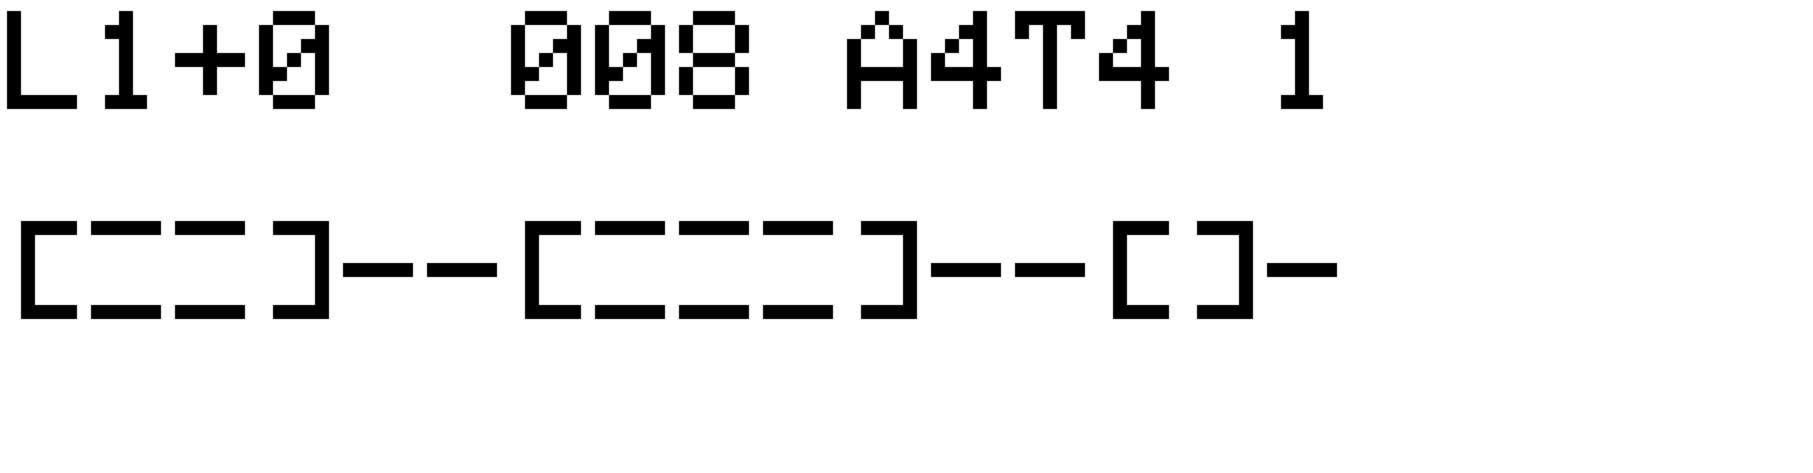
\includegraphics[scale=.40]{seq_ext_step_page.png}}\\
\\
NoteOn events notes are shown in uppercase. E.g: C 3, A#4, B 5, D#6
\\NoteOff events notes are shown in lowercase. E.g: c 3, a#4, b 5, d#6
\\\\
The first note event entered for a specific note number is always of event type NoteOn.\\
The next time the same note is entered it will automatically be placed as a NoteOff event.
\section{Encoder Assignment:}
\begin{itemize}
	\item \textbf{[ Encoder 1 ]: } Trig Condition
	\item \textbf{[ Encoder 2 ]: } MicroTiming
	\item \textbf{[ Encoder 3 ]: } Track Length
	\item \textbf{[ Encoder 4 ]: } --
\end{itemize}

\section{Program a Sequence: }
The trigger interface on the MD is used to edit the steps of the step sequence in the PolyStep Edit page.\\
\\
The notes of the Analog4 keyboard or External Midi keyboard are used to edit the note data.
\\
\begin{enumerate}
\item Press and hold the desired trigger on the MD whilst simultaneously pressing one or a maximum of 4 notes on the Analog4/Ext keyboard.
\item Adjust conditional mode or microtiming as needed using encoders 1 and 2.
\item Repeat the above for another step in the sequence, (Selecting the exact same notes). This time the notes will be entered as NoteOff events.
\end{enumerate}

\section{Clearing a sequence:}
\begin{itemize}
\item To clear the current track, press the\textbf{ [ Write ] }
\item To clear all Analog4/ExtMIDI tracks, \textbf{[Shift2 ] + [ Write ]}
\end{itemize}
\section{Rotating visible sequence:}
Each polyphonic track consists of 8 pages of 16 steps, for a total of 128 steps per track.
\begin{enumerate}
	\item Rotate the current track-page by pressing the \textbf{[Shift1] }button.
\end{enumerate}
\section{Changing track length:}
\begin{itemize}
	\item Track length is controlled by rotating \textbf{[ Encoder 3 ]}. Only steps less than the current track length are drawn.
	\item To change the lengths of all 4 polyphonic tracks simultaneously hold down \textbf{[Shift 2]} whilst rotating \textbf{[ Encoder 3 ]}.
\end{itemize}
\section{Resolution Modes:}
The polyphonic step sequencer has 2 resolution modes (high resolution and low resolution).\\
\\
By default High Resolution mode is activated and the maximum number of steps per pattern is 128 x 32th note steps, equivalent to 64 x16th note steps.
\begin{itemize}
\item High resolution mode is required, if you intend to play 16th notes in quick succession. This mode is best for live recording.
\item Low resolution mode is 128 x 16th note steps. This is perfect for slow melodic progressions where sequential 16th notes are not required
\end{itemize}
\section{Switching Between Low and High Resolution Modes.}
\textit{Press \textbf{[ Shift2 ]} followed by \textbf{[ Shift1 ]}}
